\documentclass[
	ruledheaders=section,%Ebene bis zu der die Überschriften mit Linien abgetrennt werden, vgl. DEMO-TUDaPub
	class=report,% Basisdokumentenklasse. Wählt die Korrespondierende KOMA-Script Klasse
	thesis={type=bachelor},% Dokumententyp Thesis, für Dissertationen siehe die Demo-Datei DEMO-TUDaPhd
	accentcolor=9c,% Auswahl der Akzentfarbe
	custommargins=true,% Ränder werden mithilfe von typearea automatisch berechnet
	marginpar=false,% Kopfzeile und Fußzeile erstrecken sich nicht über die Randnotizspalte
	%BCOR=5mm,%Bindekorrektur, falls notwendig
	parskip=half-,%Absatzkennzeichnung durch Abstand vgl. KOMA-Sript
	fontsize=11pt,%Basisschriftgröße laut Corporate Design ist mit 9pt häufig zu klein
%	logofile=example-image, %Falls die Logo Dateien nicht vorliegen
]{tudapub}


% Der folgende Block ist nur bei pdfTeX auf Versionen vor April 2018 notwendig
\usepackage{iftex}
\ifPDFTeX
\usepackage[utf8]{inputenc}%kompatibilität mit TeX Versionen vor April 2018
\fi

%%%%%%%%%%%%%%%%%%%
%Sprachanpassung & Verbesserte Trennregeln
%%%%%%%%%%%%%%%%%%%
\usepackage[english,ngerman, main=english]{babel}
\usepackage[autostyle]{csquotes}% Anführungszeichen vereinfacht
\usepackage{microtype}


%%%%%%%%%%%%%%%%%%%
%Literaturverzeichnis
%%%%%%%%%%%%%%%%%%%
\usepackage{biblatex}   % Literaturverzeichnis
\bibliography{thesis}
%\addbibresource{thesis.bib}


%%%%%%%%%%%%%%%%%%%
%Tabellen
%%%%%%%%%%%%%%%%%%%
%\usepackage{array}     % Basispaket für Tabellenkonfiguration, wird von den folgenden automatisch geladen
\usepackage{tabularx}   % Tabellen, die sich automatisch der Breite anpassen
%\usepackage{longtable} % Mehrseitige Tabellen
%\usepackage{xltabular} % Mehrseitige Tabellen mit anpassarer Breite
\usepackage{booktabs}   % Verbesserte Möglichkeiten für Tabellenlayout über horizontale Linien
\usepackage{makecell}
\usepackage{multirow}
\renewcommand\theadfont{\bfseries}

%%%%%%%%%%%%%%%%%%%
%Paketvorschläge Mathematik
%%%%%%%%%%%%%%%%%%%
%\usepackage{mathtools} % erweiterte Fassung von amsmath
%\usepackage{amssymb}   % erweiterter Zeichensatz
%\usepackage{siunitx}   % Einheiten


\usepackage{hyperref}
\usepackage{tikz}
\usepackage{listings}
\usepackage{subcaption}
\usepackage{amsmath}
\usepackage[justification=centering,labelfont=bf]{caption}
\usepackage{adjustbox}


%Formatierungen für Beispiele in diesem Dokument. Im Allgemeinen nicht notwendig!
\let\file\texttt
\let\code\texttt

\usepackage{pifont}% Zapf-Dingbats Symbole
\newcommand*{\FeatureTrue}{\ding{52}}
\newcommand*{\FeatureFalse}{\ding{56}}

\lstdefinelanguage{JavaScript}{
  morekeywords=[1]{break, continue, delete, else, for, function, if, in,
    new, return, this, typeof, var, void, while, with, await, async, case,
    catch, class, const, default, do, enum, export, extends, finally, from,
    implements, import, instanceof, let, static, super, switch, throw, try},
  % Literals, primitive types, and reference types.
  morekeywords=[2]{false, null, true, boolean, number, undefined,
    Array, Boolean, Date, Math, Number, String, Object},
  % Built-ins.
  morekeywords=[3]{eval, parseInt, parseFloat, escape, unescape},
  sensitive,
  morecomment=[s]{/*}{*/},
  morecomment=[l]//,
  morecomment=[s]{/**}{*/}, % JavaDoc style comments
  morestring=[b]',
  morestring=[b]",
  morestring=[b]`
}[keywords, comments, strings]

\lstset{
  language=JavaScript,
  basicstyle=\ttfamily,
  numbers=left
}

% these words should not by hyphenated
\hyphenation{postMessage}
\hyphenation{setTimeout}
\hyphenation{setInterval}



\begin{document}

\Metadata{
	title=Analysis of Methods for Background Execution in Modern Web Applications,
	author=Yannick Reifschneider
}

\title{Analysis of Methods for Background Execution in Modern Web Applications}
\subtitle{Analyse von Verfahren für Hintergrundausführung in modernen Webanwendungen}
\author[Y. Reifschneider]{Yannick Reifschneider}%optionales Argument ist die Signatur, 
\reviewer{Dipl.-Inf. Nikolay Matyunin \and Prof. Dipl.-Ing. Dr. Stefan Katzenbeisser}%Gutachter

%Diese Felder erden untereinander auf der Titelseite platziert. 
%\department ist eine notwendige Angabe, siehe auch dem Abschnitt `Abweichung von den Vorgaben für die Titelseite'
\department{inf} % Das Kürzel wird automatisch ersetzt und als Studienfach gewählt, siehe Liste der Kürzel im Dokument.
\institute{Security Engineering Group}
%\group{Security Engineering Group}
%\addTitleBoxLogo{SecEng_white}

\submissiondate{\today}
\examdate{\today}

%\tuprints{urn=1234,printid=12345}
%\dedication{I dedicate this thesis to my deceased sister Kimberly whose support and encouragement enriched my life and inspired me to pursue and complete my studies.}

\maketitle

\begin{abstract}
  The world wide web today is not only used for serving static pages of information but it is also used as a platform for sophisticated web applications. These web applications may be left opened for long durations during everyday computing activities. Other reasearch shows that there are many attacks against the web browser executed from malicous web sites. Some of these attacks assume a long uninterrupted timespan for execution, for example cryptocurrency miners or exploits targeting hardware-based vulnerabilities. Therefore, these attacks greatly benefit from being executed from web applications which are left opened for a long time on the victims computer. However, most web browsers limit the time a web site can execute code, when the web site is not in focus for energy conserving reasons. Hence we try to answer the question whether the background execution limitations prevent those attacks.

  In this thesis we analyse modern browsers regarding their behaviour of JavaScript code execution in background tabs. We show that the energy conserving limits of background code execution of most browsers can easily be circumvented. We discuss and explain how the circumvention methods work and how browsers behaviour differ. For this research we developed a framework for comparing and analysing different methods for background execution. This framework allows expansion for newly discovered methods as well as review of existing methods for newer browser versions.

  With the findings from our research, we performed a dynamic analysis of popular web sites to measure their code execution in the background and determine if they use the limit-circumventing techniques we identified. The result of this analysis shows that some web sites do unnecessary circumvent the browser limits by one or more methods we explained.

  To conclude, we discuss potential changes to browsers to prevent background code execution for web sites without explicit user consent.
\end{abstract}

\tableofcontents

\newpage

\chapter{Introduction}
\label{chap:introduction}

Web technology received rapid advances in the last years. Nowadays, many websites not only deliver static information in form of text and images. Instead, modern web sites implement complex logic by executing JavaScript code on the client. This allows web sites to build highly dynamic applications which compete with traditional software products. For many of the standard business applications like an e-mail client, a word processor or even a bitmap graphic manipulation software there exist alternatives \cite{gmail}, \cite{office365-online}, \cite{photopea}, which are developed using web technologies and are accessed via a modern web browser.

Some reasons for the rise of popularity of web applications are that the web platform is providing more powerful APIs every year and the performance of browsers is drastically increasing, thus CPU intensive tasks are feasable to be implemented as web application. Developing a web application instead of traditional software has also many benefits for the developers and publishers of said software. Web applications do not need installation. They just require a modern web browser which comes preinstalled with any common operating system or mobile device. Users always use the latest version, because it is not installed to the users hard drive, thus support and maintanance costs are reduced. Visiting a web site to try out a piece of software is a much smaller hurdle to overcome than downloading, installing and running a piece of traditional software. These are some reasons which make the web a popular platform for development of new applications.

The web browser is a fundamental application on most personal computing devices and web browser usage is ubiquitous in everyday computing activities, because many modern applications are implemented as web apps. Also, users often use a browser with many tabs open at once \cite{weinreich2008not}. As such, browser vendors are encouraged to conserve as much energy as possible to enable users on battery powered devices, such as mobile phones or notebooks which are not tethered to a power outlet, a longer usage time. For maximum energy efficiency, all tabs in the background should eventually be halted completely, and only woken up when the page is moved to the foreground again. Suspending all background tabs is the stated goal of browser vendors \cite{chrome-background-tabs-roadmap}. However, this change in behaviour is not yet implemented due to missing alternative APIs enabling the major use cases, which require background execution. Web apps, which need regular CPU time are sites, which notify the user about new content such as a news site or a social network, a web application which plays audio or video, or a web video conference application. For the time being, browsers only \textit{limit how often} web sites can schedule new work when a web site is not in focus to not break existing sites which are performing background tasks.

Other research shows that there are attacks against the web browser, which assume or benefit from some form of background execution. When a malicious entity gains script execution on a popular web site it could perform several attacks. Consider a cryptominer which uses the CPU power of the victims computer to calculate crypto currency for the attacker as described by Rüth et al. \cite{rueth2018digging}. Cryptominers would benefit greatly when they could expand their runtime to background tabs. Another example for malicious use of background execution is the participation in a browser based botnet as outlined by Grossmann and Johansen in \cite{grossmann2013million}. Likewise, this attack scenario benefits from constant ability to perform background execution, too. However, it is not clear if the energy-saving mechanisms put in place by modern browsers prevent these kind of attacks or if script execution in background tabs is as utilizable as in foreground tabs.

  \section{Goals of our research}

  The goals of our research are threefold: First, we want to analyse how browsers throttle tasks in background tabs. Second, we try to find methods to circumenvent the throttling mechanisms put in place by browser vendors. And third, we analyse popular web sites to confirm whether these methods are used to actively or inadvertently circumvent the browser throttling. However, we are not investigating what these web sites do in the background, merely if and how long background tasks are executed.

  With this research, we contribute the answer to the question whether the current energy-saving mechanisms implemented by browsers are suitable to protect users from malicious background activites on rogue web sites or how the energy-saving mechanisms can be circumvented for malicious use.

  \section{Organization of this thesis}

  This thesis is organized into the following chapters:

  \begin{description}
  \item[Chapter 2] describes the basic principles of web scripting and how the JavaScript language handles tasks and concurrency.
    
  \item[Chapter 3] gives an overview of other research related to our field of study. We compare our research to prior work and highlight possible attacks targeting browsers which assume some form of continous execution time.
    
  \item[Chapter 4] describes methods for performing tasks in background tabs. We analyse how each browser behaves in regard to their throttling mechanisms to each method and how various browser implementations differ.
    
  \item[Chapter 5] is about dynamic analysis of background execution of popular web sites. We explain how automated profiling of these web sites was conducted and we describe the results of the analysis.
    
  \item[Chapter 6] summarizes the result of our research and discusses propsed changes to the behaviours of browsers to protect users from unwanted background execution.
  \end{description} 

  
  \newpage
  \chapter{Background}
  
  The development of modern web applications is done with JavaScript code, which gets embedded in the resources of the web site and is executed by the browser. The JavaScript language was originally designed as an extension to HTML (Hypertext Markup Language) and CSS (Cascading Style Sheets) which form the foundation of the world wide web. The goal was to enable simple user interaction with web pages like validation of user-entered form input. Although nowadays it is used for much more sophisticated web applications, the basic principle of the web did not change since: When a user visits a web site, the browser downloads all resources belonging to this web site, like HTML, images and also JavaScript code. These scripts are run to build up the complete website. When a user visit a web page and did not disable JavaScript execution, they implicitly allow this web site to execute code on their machine.

  Most desktop browsers also provide an alternative to run client applications on users machine via plugins, such as Java Applets, Flash or Silverlight. However, these plugins are usually not supported by mobile browsers and the usage steadily declined since smartphones and mobile browsers became widely adopted. Today JavaScript is the dominating technology for browser based applications \cite{browser-plugin-usage}.

  JavaScript is a scripting language. As such, it is not compiled to native machine code but it requires an interpreter which parses and executes the JavaScript code at runtime. All major browsers include an JavaScript interpreter to correctly display modern web sites. The HTML5 specification describes how JavaScript engines have to interoperate with the browser and which APIs the browser must expose to JavaScript code which is embedded in web sites \cite{html5-specification}.
  In the following sections we describe how browsers run JavaScript code and how concurrency and long running tasks are handled in JavaScript.

  \section{The JavaScript execution context}

  Each browser tab creates a browsing context which allows interfacing with the opened web site. JavaScript code embedded in the web site can either be executed in this browsing context or another context created by this web site, e.g. a web worker. In this thesis we define \textbf{execution context} to refer to both a browsing context and other contexts in which JavaScript code is executed in.

  A JavaScript execution context is organized into a task queue, an event loop, a stack and a heap. We briefly describe each in the following paragraphs. Detailed information is available in \cite{mdn-event-loop}.

  \begin{description}
  \item[Task queue] The task queue defines a list of tasks which should be executed by the JavaScript runtime. A task consists of a callback function and optional arguments to this callback function.
  \item[Event loop] The JavaScript runtime implements an event loop which processes the task queue. During the event loop the runtime waits for tasks to be added to the task queue. When the task queue is not empty, the event loop removes the first task from the queue and executes its corresponding callback function with the provided arguments. This procedure is repeated until the task queue is empty at which point the event loop transitions to waiting for new tasks again.
  \item[Stack] The stack is comparable to a call stack in other programming languages like Java or C. When a callback function from the task queue is executed, it creates a frame on the stack. Each function call inside the callback function also creates a stack frame. When a function returns, its frame is removed from the stack. A task from the task queue is finished when the stack is empty.
  \item[Heap] The heap is a memory region for long living objects which are not destroyed after the execution of a single task.
  \end{description}

  When a JavaScript task is running, it is guaranteed to behave as if the execution of that scripts is completely serialized \cite{html5-specification}. This also ensures that all variables cannot be changed during the execution of a task. This is in contrast to many other programming languages like Java or C, where another thread can mutate variables at any time. To guarantee this behaviour, the JavaScript runtime in the web browser has to wait for tasks to finish before it can continue rendering the web page, since the JavaScript task has access to the browser internal state and Document Object Model (DOM). The DOM describes the representation of a web page and provides an API for manipulation of the element tree and registration of event handlers. Due to JavaScript code having access to these internal structures, tasks should be as small as possible to ensure responsiveness of the browser \cite{chrome-rail-model}. If a JavaScript task takes a long time to complete (i.e. it is executing an infinite loop) most browser show a warning to the user that a script is slowing down the website. Figure \ref{fig:blocking-script} shows how Firefox displays this dialog. The user has the option to stop the task or wait for the task to finish.

  \begin{figure}
    \centering
    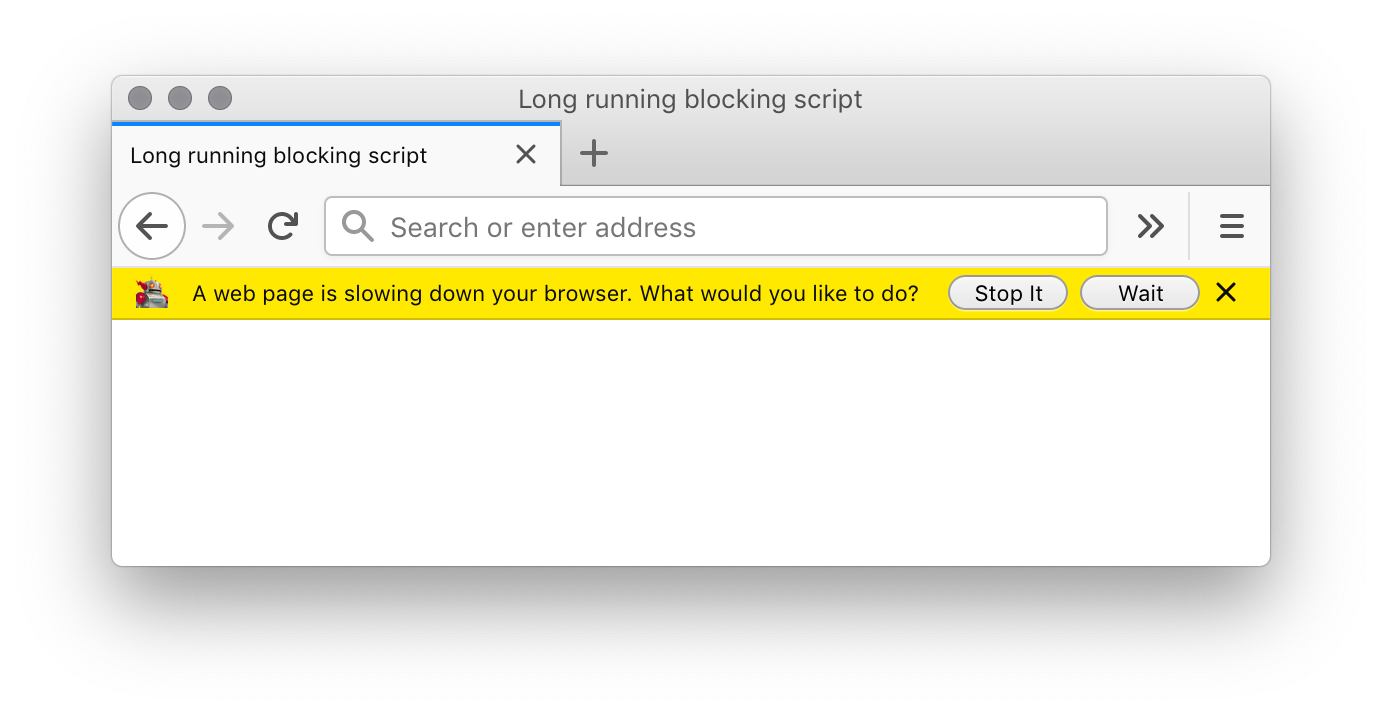
\includegraphics[width=0.6\textwidth]{images/blocking-script.png}
    \caption{Firefox asking the user whether to wait for or to stop a long running blocking script}
    \label{fig:blocking-script}
  \end{figure}

  Tasks can be added to the task queue by registering event listeners for events, for example in response to a user clicking a button. When this event occurs, the runtime then adds a new task to the task queue. Tasks can also be added by JavaScript code itself for example by using a timer.
  
  \section{The JavaScript concurrency model}
  
  The JavaScript language does not support explicit multi threading. The execution context of each browser tab is tied to the rendering of the page, as explained in the sections before. As long running JavaScripts tasks block the rendering of the web page, calls to potentially long running functions are almost never blocking. Instead, they register a callback function to be called when the result of function returns. As soon as the result of the called function becomes available, the runtime creates a new task in the task queue with the registered callback function and the result as a parameter for the callback. Due to this API design, scripts are splitted into small tasks, whenever a long running function has to be called. The long running functions, which are performed by the runtime, can happen in parallel. The serializability guarantee of JavaScript only holds to each task. Therefore, the browser can perform rendering activities or start new tasks while waiting for the results of the callback tasks.

  Consider the following example code performing a web request.
\begin{lstlisting}
function doNetworkRequest() {
  fetch('https://www.example.com')
    .then(function callback1(response) {
      response.text()
        .then(function callback2(text) {
          console.log('Network request returned:', text);
        });
    });
}
\end{lstlisting}
  In the function \texttt{doNetworkRequest()} the call to \texttt{fetch()} performs a network request. The call to \texttt{fetch()} is an example of a long running function accepting a callback via the returned \texttt{then()} method. The \texttt{callback1()} function in line 3 is invoked with the response from the network call as a parameter when the response becomes available. The call to the method \texttt{text()} of the response object is also a callback accepting function. Each \texttt{function} declaration would be invoked as an indivual task by the runtime. The serializability guarantee holds for each function individually, but not the script as a whole.

  In summary, a JavaScript tasks is the atomic unit of execution. The execution of tasks are serializable. Most web scripting is composed of many small tasks which are executed by the browser when an event happened or the result of another function becomes available.
  
  \section{Web workers}
  \label{sec:web-workers}

  Web workers were an addition to the HTML5 specification to overcome the limitation of long running tasks blocking the rendering of the browser. Unlike tasks executed in the main browser context, web workers create a new execution context which is \textit{not tied} to the browser rendering. Long running, undividable tasks can be executed in the worker context without blocking the rendering. They do not share variables or resources with the main execution context. Therefore, the worker context does not have access to the DOM of the web page, because that would introduce shared memory between the worker and main context which would invalidate the runtime guarantees of the JavaScript specification. However, other resources, such as network requests that are independent from the main context, are available to the worker context. The web worker and main thread context can communicate by passing messages to each other which are handled by their respective event loops. This allows the result of a calculation happening in the worker context being passed to the main context and then being visualized to the user by appending the result to the DOM.

  
  \section{Dynamic analysis of JavaScript code}

  

  
  \newpage
  \chapter{Related work}


  
  At the same time the revenue model for many websites is advertising. Websites include third party JavaScript from ad networks, which display ads and track impressions. The included code can be controlled by the advertiser. For a malicous entity, it is therefore possible to include JavaScript on reputable websites just by paying for the ad impression. This method of distribution for malicous script is known as malvertising\cite{wiki:malvertising}.
 

  Nevertheless, there are numerous activities which malicous entities could perform with access to a web site with high number of visitors.

  \begin{itemize}
  \item The attacker could inject a browser crypto-currency miner to convert electricity of the website visitors into crypto currency. The existance of crypto currencies such as Monero, which uses proof of work algorithm, which is inefficient to calculate on custom hardware, makes the browser a viable target for such mining. Existing implementations of Monero miners implemented in web assemlby are available for this attack.
  \item The browser could be used as a compute node in a botnet, which can be used for DDoS attacks or for cracking hashed passwords. Grossman et al.\cite{grossmann2013million} show that these attacks can be used with standard web technologies and not exploiting any weaknesses.
  \item The computer of the visitor itself could be compromised by using exploits of the browser or the underlying system itself. Attacks which exploit hardware weaknesses such as Spectre\cite{Kocher2018spectre}, which could allow an attacker to read memory space of other browser tabs, could expose sensitive informations such as passwords or banking information of the uses. Rowhammer\cite{rowhammer} attacks could even persistently infect the users system. These exploits usually need quite some time to be successful and could benefit from constant background execution in a background browser tab.
  \end{itemize}

  \textbf{TODO: restructure to formal text instead of bullet points}

  \begin{itemize}

  \item Papadopoulos et al.\autocite{papadopoulos2018truth} analyses the if Cryptocurrency miners are a viable alternative to traditional ad serving as a revenue possibility for web sites. They come to the conclusion, that cryptocurrency mining is more profitable when a user stays longer then 5.3 minutes on the website. When permanent execution of a crypto miners are possible in background tabs, then this time could easily be achieved.

  \item Papadopoulus et al.\cite{papadopoulos2018master} show that browsers can be infected with malicous service workers to act as a puppet in a botnet. Their method for persistence requires an implementation of a draft proposel HTML5 API, which is not implemented in mainstream browsers yet. They focus in their research on service workers, which are independent of browser tabs, but poses other limitations. Our research instead focuses on web sites which are not user visible, i.e. in an inactive tab.   

    
  \item Measurements of existing popular websites is done for privacy related as well as security releated research. Engelhardt et al.\cite{englehardt2016online} for example developed the OpenWPM framework for doing privacy measurements on million of websites. This framework is also used for ...

    Security related analysis of existing webpages are done for example: to measure the use of third party script inclusions\cite{nikiforakis2012you}, to assess the security claims provided by third party security seal providers\cite{van2014clubbing} or to study malware distributed via ad networks\cite{zarras2014dark}.


  \item Pan et al. analyse the feasability to use the browser of website visitors for offloading large computing tasks\cite{pan2015gray}. They termed this usage of distributed data processing gray computing, because it can be done without the users explicit consent, for example while the users are watching video streams. Their research focus is the performance of web workers and the cost effectiveness in comparison to cloud computing offerings. Our research complements the findings of Pan, because they could allow grey computing even when the user is consuming other web sites.

    
  \end{itemize}


  
  \newpage
  \chapter{Analysis of background execution methods}
  \label{chap:analysis}

  As we have shown in chapter \ref{chap:introduction} of this thesis, there are numerous incentives to execute code in background browser tabs. In contrast, browsers vendors are motivated to limit the energy impact of JavaScript code in background tabs as much as possible to prolong the battery life of the users device. To assess the behaviour of the browser throttling mechanisms, we developed a framework to compare different methods for achieving background code execution.

   In this thesis we define \textbf{background tab} to mean a browser tab which is not currently selected as the focused tab, i.e. another tab is currently visible in the browser window, and \textbf{background execution} means JavaScript task execution in a background tab.

  Currently, the browser market is dominated by only three different browser engines. Browser engines form the foundation of a web browser and include a rendering and a scripting engine. Blink, the browser engine of Chrome which is also used in Opera and new versions of Edge. Safari for macOS and Mobile Safari for iOS use the WebKit browser engine. WebKit is also used for every other browser available in the iOS operating systems application store (App Store), because every application displaying web content has to use the system-provided WebKit framework to be in accordance with the App Store Review Guidelines \cite{apple-app-review-guideline}. Applications that to not comply with these guidelines are not permitted in the App Store. The third browser engine is Gecko used by Firefox for desktop and for Android. Of the global world wide web usage, these three browser engines cover 90 \% of the market share according to \cite{statcounter-global-browser-market-share}. Based on this data, we decided to focus our analysis on the following desktop browsers:

  \begin{itemize}
  \item Google Chrome 76
  \item Mozilla Firefox 69
  \item Apple Safari 12.1.2
  \end{itemize}

  For mobile browsers we evaluate these browsers:

  \begin{itemize}
  \item Google Chrome for Android 76
  \item Firefox for Android 68
  \item iOS 12.4.1 Mobile Safari
  \end{itemize}

  This selection covers the most used browsers for each browser engine on desktop and mobile.

  \section{Methodology}

  In the following sections we look at different methods for scheduling JavaScript code when the tab is in the background. We describe how each browser behaves when this method is used to execute JavaScript code in the background and we use our measuring framework to compare the browser behaviour for each method.

  The measuring framework takes one parameter to tune the measuring. With this parameter we can define the workload in milliseconds. This time defines how long a simulated task should perform uninterrupted work. When this work is performed on the JavaScript main execution context then the browser is unresponsive for this amount of time, until the simulated workload finished and yields back to the event loop. Google Chrome advises to keep the execution time of all tasks under 50 ms as this duration is being percieved as immediate to the user \cite{chrome-rail-model}. For our analysis we measure each method with two workload times for each browser, once for the recommended 50 ms workload and once for a long 1000 ms workload. The measurement is started automatically when the website page is moved to the background and stopped when it is visible again. The framework uses the Page Visibility API \cite{mdn-page-visibility} for determining the current page visibility.

  The following code snippet illustrates how the measuring framework is used.
\begin{lstlisting}
const workloadDurationMs = 1000;
const measurement = new Measurement(function setup() {
  let intervalId;
  return {
    start(simulateWork) {
      intervalId = setInterval(simulateWork, 0);
    },
    stop() {
      clearInterval(intervalId);
    }
  };
}, () => workloadDurationMs);
\end{lstlisting}
  In this example we measure the invocations of tasks scheduled with \texttt{setInterval()}. The measuring frameworks takes a setup function which must return an object with a \texttt{start()} and \texttt{stop()} method. The \texttt{start()} method is called when the browser tab is being moved to the background and should start scheduling the \texttt{simulateWork} callback function as fast as possible. The \texttt{stop()} method is called when the tab moves to the foreground again and should stop the scheduling. The \texttt{simulateWork} callback function of the measuring framework simulates calculation for the amount of time passed as second argument to the \texttt{Measurement} class constructor and records its invocation time for later analysis.

  To test the chosen browsers in an automated way, we developed a script using Selenium WebDriver \cite{webdriver}. WebDriver lets us automate various browsers using a common API. In our automation script, we open our analysis page which embeds our measuring framework and start the benchmark by opening a new empty browser tab. After a fixed amount of time, we close the empty browser tab to make the analysis page visible again and thus stop the measuring. This procedure is repeated for every browser with every test method and the two defined workload times.

  After the benchmarking for one scenario is complete, the measuring framework produces a report for downloading the recorded invocations in the background. The recorded data includes the time since the web page moved to the background, the time since the last invocation and a computed average CPU usage for each invocation. This computed average CPU usage is derived from the last invocation time $\Delta t_{last invocation}$ and the simulated work load duration $t_{work duration}$  with the following formula:

  \begin{equation*}
    \text{CPU}_{avg} = \frac{t_{work duration}}{\Delta t_{last invocation}}
  \end{equation*}

  Afterwards, we can plot the computed CPU usage over time and compare different browsers for each scenario.

  \section{Methods for background execution}
  \label{chap:methods}

  In this section we describe methods for scheduling tasks and we describe if and how each browser throttles or suspends these tasks when they are executed in background tabs.
  
  \subsection{Timer tasks}
  \label{sec:timer-tasks}

  The default method to schedule new tasks for execution is to use the function \texttt{setTimeout()} or \texttt{setInterval()} which are available in the main and the worker execution context. These methods take at least two arguments. The first is the function which should be scheduled as a task. The second argument is the time in milliseconds to wait before the task should be executed. As this is the most straighforward way to schedule tasks, this method might be the one which gets throttled the most. In particular, the HTML5 specification for timers \cite{whatwg-timers} even explicitly defines an optional waiting time which is user-agent defined to allow for optimization of power usage. Also, when \texttt{setTimeout()} calls are nested or \texttt{setInterval()} repeats the fifth time, the minimum waiting time is incresed to be 4 ms. We used our measuring framework to determine the browser behaviours with background timer tasks. The results for desktop browsers are shown in figure \ref{fig:timer}.

  Google Chrome throttles timers for background tabs. Since Version 11, timers are batched at most once a second \cite{chrome-background-tabs}. We observed and confirmed this behaviour with our measuring framework. The batching is made visible in figure \ref{fig:timer} by the short peaks of CPU usage. Timer batching or coalescing is used to reduce the number of times the CPU has to be woken up from low power mode. Most modern CPUs have a low power mode which consumes significant less energy than the high power mode. Switching modes also costs energy. Therefore, it is better for energy efficiency to switch modes as few times as possible. This can be achieved by coalescing timer tasks. Since Version 57 Google Chrome also uses a budget-based timer throttling. Budget-based timer throttling works by introducing a timer budget for every background tab. When the web site is in the background for longer than 10 seconds, the budget is considered for. Every scheduled timer task is only executed when the budget for this page is greater then zero. The runtime of the task is subtracted from the budget. The budget regenerates for 0.01 seconds per second \cite{chrome-background-tabs}. We also observed and confirmed the timer throttling with our framework, as shown in figure \ref{fig:timer}. For the 50 ms tasks the budget was high enough to run for an additional 12 seconds before the budget was negative for the first time, whereas the 1000 ms tasks depleted the budget before the 10 second mark. This budget based throttling has multiple implications for background tabs. First, it allows for sudden bursts in computing time when these burst are infrequently engough to let the budget replenish. The budget regenereates continously at a low rate but can be depleted in a very short amount of time. Second, background pages which want to use continous computation time are limited to an average of 1 \% of CPU usage over time, because the budget regenerates at a rate of 0.01 seconds per second. Chrome for Android behaves just as its desktop counterpart except that background tabs are only active for 5 minutes \cite{chrome-android-suspend}. After that, the tab is completly suspended and only woken up when the tab is in focus again.

  Firefox employs similiar throttling mechanisms to the ones from Google Chrome \cite{mdn-page-visibility}. Still, we observed that the details of the Firefox implementation differ slightly. When a page is in the background, Firefox invokes timers at least one second after the last timer finished. This is in contrast to Chrome's throttling to one invocation per second. The difference is most visible when the task duration is one second. With Chrome's throttling implementation the next task fires immediatly, whereas Firefox waits an additional second, before the next task is executed. This is also visible in figure \ref{fig:timer}. Firefoxs average CPU usage for 1000 ms tasks is shown with 50 \% before the budget throttling is activated. Another difference is that the budget based timer throttling is used after a page is in the background for 30 seconds instead of 10 seconds for Google Chrome. Additionally, Firefox caps the page budget at a minimum of -150 ms and a maximum of 50 ms. That means that Firefox does not allow bursts of smaller tasks with a combined duration larger than 50 ms, because the budget never increases above that limit. However, individual, longer lasting tasks do not overdraw the budget more then -150 ms. This behaviour favors tasks which are longer than 150 ms. For example, a repeated task with a duration of 1000 ms only needs to wait for 15 seconds, before the budget is positive again in Firefox, whereas a task with the same duration would have to wait for 100 seconds in  Chrome. Firefox also employs additional throttling to known tracker scripts, such as Google Analytics. Invocations of tasks of these tracker scripts are limited to at most once every 10 seconds \cite{mdn-tracker-throttling}. Firefox for Android behaves exactly like the desktop version. We could not detect or observe further energy optimizations in the mobile port of Firefox. 

  Safari's throttling behaviour is different from that of the other two browsers. Scheduled tasks in background pages get invoked by Safari in increasing intervals. This ensures that the CPU usage for background pages decreases much more rapidly then the CPU usage of the same page in Chrome or Firefox. Safari also coalesces timer calls to prevent a lot of small periodic wake ups of the CPU. Instead of that, multiple timers are invoked consecutivly to let the CPU move to an energy saving state for a longer period. We observed the increasing intervals in our measurements up to a limit of three minutes between invocations, but we could not determine the exact growth rate of the increases. We analysed the WebKit source code and determined that the increase grows exponential \cite{webkit-timer-increases}. Mobile Safari completely disables the invocation of all timers as soon as the page moves to the background. It is the most restricting browser of all we assesed.
  
  
  \begin{figure}
    \begin{subfigure}[t]{0.5\textwidth}
      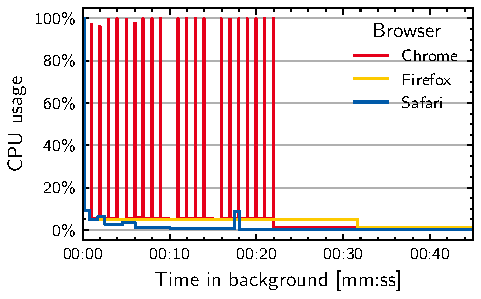
\includegraphics[width=\textwidth]{images/timer-50.pdf}
      \caption{50 ms task duration}
    \end{subfigure}
    \hfill
    \begin{subfigure}[t]{0.5\textwidth}
      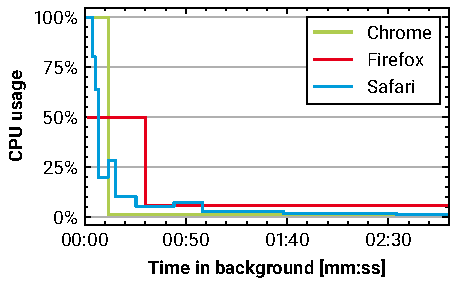
\includegraphics[width=\textwidth]{images/timer-1000.pdf}
      \caption{1000 ms task duration}
    \end{subfigure}

    \caption{CPU usage over time for continuously scheduled timer tasks in background tabs}
    \label{fig:timer}
  \end{figure}

  \subsection{Timer tasks with active WebSocket / AudioContext}

  Browser vendors try to strike a balance between throttling background pages as much as possible to conserve energy and keep the foreground tab more responsive and not breaking existing web applications. As backwards compatibility is an important factor for users, some browsers reduce their throttling when they detect that a web application might need more background processing time. The detection that a web site needs more processing time is difficult though. Due to the dynamic nature of JavaScript, static analysis of JavaScript is very difficult. Therefore, browsers use simple heuristics, to determine if their default throttling should be reduced. One such heuristic is the presence of an open WebSocket connection \cite{mdn-websocket} or media playback with the AudioContext API \cite{mdn-audiocontext}. Again, we measured and observed the behaviour with our measurement framework. The results of desktop browsers are shown in figure \ref{fig:websocket}.

  Chrome disables the budget-based throttling when a web site has either an active WebSocket connection open or plays audible sounds. Playing silent music does not count as audible music playback though \cite{chrome-background-tabs}. This behaviour could be misused to get more processing time for JavaScript tasks. Playing a audible sound or opening a WebSocket connection work equally in preventing the budget-based throttling, but they differ hugely in how noticeable they are to the user of the web page. Playing audio is obviously audible and marks your tab with a speaker icon in the tab bar. This is a convenience feature for users to quickly find out, which tab is producing the sounds. Additionally, playing audible sound without explicit user consent is frowned upon by many internet users. Actually, Chrome prevents automatic playback of audio unless the user has interacted with the site before or the web site is explicitly whitelisted as a web site with a high media engagement index \cite{chrome-media-engagement-index}. This index is used to determine if a web site can allow audible media autoplay and is generated by the user's browsing history. On a new installation of Chrome, this list is prepopulated with over 1000 sites which Google determined to have a high average media engagement index of all Chrome users \cite{chrome-autoplay}. However, opening a websocket connection is invisible to the user and requires no user confirmation. Chrome on Android behaves exactly the same as Chrome for desktop except for the five minute limit as described in section \ref{sec:timer-tasks}.

  Firefox also disables the budget-based throttling when a WebSocket connection is active, but the limitation of one task invocation per second stays intact. However, Firefox does completely disable all timer limits when an AudioContext was created on the web site since Firefox version 51 \cite{firefox-audiocontext-exemption}. We could observe and replicate this behaviour on Firefox for desktop as well as Firefox for Android, even when no audible audio was playing at all. Creating an AudioContext does not require special user permission and allowed us to saturate the main thread with an average CPU usage close to 100~\%. With this method we can completely bypass all energy conserving methods on Firefox.

  Safaris behaviour does not change when a WebSocket connection is active or an inaudible AudioContext was created, neither for Safari for Mac nor for Mobile Safari for iOS.

  \begin{figure}
    \begin{subfigure}[t]{0.5\textwidth}
      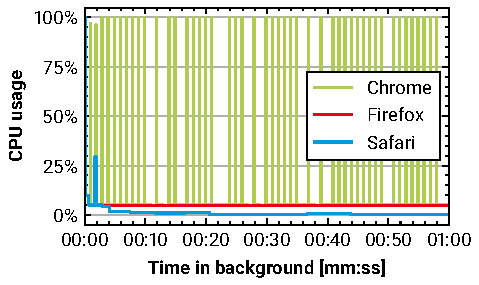
\includegraphics[width=\textwidth]{images/websocket-50.pdf}
      \caption{50 ms task duration}
    \end{subfigure}
    \hfill
    \begin{subfigure}[t]{0.5\textwidth}
      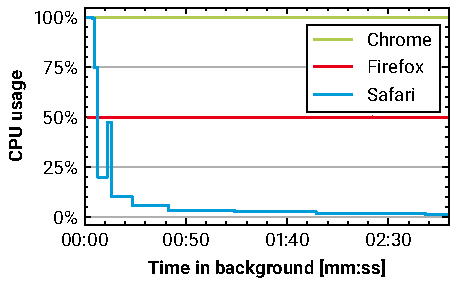
\includegraphics[width=\textwidth]{images/websocket-1000.pdf}
      \caption{1000 ms task duration}
    \end{subfigure}

    \caption{CPU usage over time for continuously scheduled timer tasks in background tabs with an open WebSocket connection}
    \label{fig:websocket}
  \end{figure}



  \subsection{\texttt{postMessage()} tasks}

  Besides \texttt{setTimeout()} or \texttt{setInterval()} there exists another API for putting tasks into the task queue. The function \texttt{postMessage()} available on the main and worker context allows for communication between windows of different origins or between main and worker context \cite{mdn-postmessage}. As each window or worker has its own execution context, the communication between those must happen explicitly via \texttt{postMessage()} calls. The receiving context has to actively register for receiving these events. After that, a call to \texttt{postMessage()} with the receiver set to a window or worker that registered for the event adds a new task to the task queue of the receiving execution context. The execution of tasks, which are created with this method, are not subject to the throttling limits as explained in the timer tasks section \cite{zero-delay-timeouts}. This is also true when the \texttt{postmessage()} call is sent and received from the same execution context.

  We analysed this method of scheduling tasks with our measurement framework and we observed that all desktop browsers do not throttle or otherwise limit the execution of task created via \texttt{postMessage()}. This allows a web site to fully utilize background execution. Chrome and Firefox allow this method to run indefinitely. However, we observed that Safari detects web pages using significant energy and terminates the complete page after around eight minutes in the background. Figure \ref{fig:significant-energy} shows how Safari is communicating the termination of a web site to the user. However, we could not use this method to achieve background execution in Mobile Safari, as it completely suspends the execution of tasks of background tabs.

  \begin{figure}
    \centering
      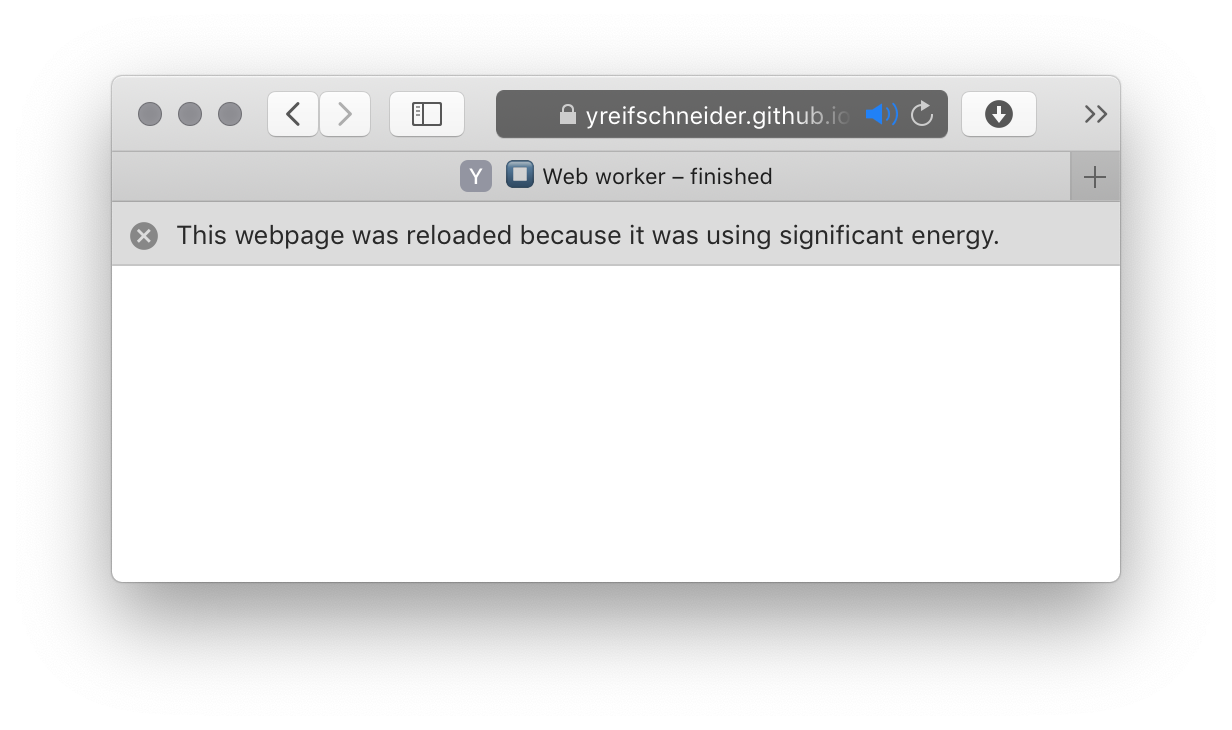
\includegraphics[width=0.5\textwidth]{images/significant-energy.png}
    \caption{Safari showing a warning about a web site after it was termined because of significant energy usage}
    \label{fig:significant-energy}
  \end{figure}

  
  \subsection{Web workers}

  As explained in section \ref{sec:web-workers}, web workers allow us to spawn a seperate execution context which behaves different than the main execution context \cite{mdn-worker}. Worker contexts are also treated differently by browsers with regard to background timer throttling. Timers created with \texttt{setInterval()} or \texttt{setTimeout()} inside the worker context are not subject to the throttling when the corresponding web page moves to the background. This fact is used by the library worker-timers \cite{worker-timers}, which implements a broker and scheduler for timer tasks in web workers for explicit use in background tabs. The scheduler component runs inside the web worker context, whereas the broker is run from the main execution context and dispatches messages when a timer was created or cleared via \texttt{postMessage()} calls to the worker context. The scheduler then creates an appropriate timer inside the worker context. When the timer fires, the scheduler posts a message to the main thread which then calls the scheduled function. Through this indirection the main thread can schedule timers with the worker-timers library as if it was using the native window timers, but without the background timer task limits. We created a test case with our measuring framework to find out how each browser behaves with this workaround.
  
  Chrome, Firefox and Firefox for Android do not throttle timers in web worker contexts in background tabs at all. This means you can max out the main thread context with the worker-timers library for indefinite time. Chrome for Android also doeas not throttle the worker timers, but it suspends background execution after five minutes. Safari does also not throttle timers in web worker context for background tabs, but, again, it detects significant energy usage and terminates the page after around eight minutes constant high CPU usage. Mobile Safari does suspend timers in worker context in background tabs, thus not allowing background execution with this method.
  
  
  \section{Summary}

  In this chapter we analysed the behaviour of background tabs for desktop and mobile browsers. We saw that all browsers employ a timer throttling when the page is in the background. Chrome and Firefox use a budget-based timer throttling approach, whereas Safari increases the time between timer calls with every invocation. The timer throttling of all browsers can be circumvented by using the \texttt{postMessage()} or by using web workers. Additionally, Chrome's budget-based limits can be disabled by creating a WebSocket connection and the all timer limits in Firefox can be disabled by opening an inaudible AudioContext. With all circumvention methods, we can saturate the main thread for an infinite amount of time in Chrome and Firefox. Only Safari detects continuous high CPU usage and terminates the page when it is using significant energy. Table \ref{tab:desktop-browser-background} summarizes the findings for desktops browsers.

    The behaviours of Mobile Safari and Chrome for Android differ in some aspects to their desktop counterparts. Mobile Safari completely suspends background tabs as soon as the user switches to another tab. Chrome for Android limits the scheduling of tasks to a maximum of five minutes when the page is in the background. However, we could not detect a change of behaviour in regard to background exection in Firefox for Android compared to the desktop version of Firefox.

  \begin{table}
    \centering
    \begin{adjustbox}{angle=90}

      \begin{tabularx}{\textheight}{ p{3cm} | X | X | X }
        \toprule
       \thead{Method}              & \thead{Chrome} & \thead{Firefox} & \thead{Safari}                   \\
      \midrule
      Timer tasks                  & Coalesced invocations at most once per second. Budget-based throttling after 10 seconds in background. Budget regenerates at 0.01 seconds per second.
                                   & Next invocation at least one second after last invocation. Capped budget-based throttling after 30 seconds in background. Budget regenerates at 0.01 seconds per second.
                                   & Coalesced invocations. Time between invocations increases exponentially up to a maximum of 3 minutes          \\
      \midrule
      Timer tasks with WebSocket
                                   & Coalesced invocations at most once per second. No budget-based throttling.
                                   & Next invocation at least one second after last invocation. No budget-based throttling.
                                   & Coalesced invocations. Time between invocations increases exponentially up to a maximum of 3 minutes.          \\
      \midrule
      Timer task with AudioContext
                                   & Coalesced invocations at most once per second. Budget-based throttling after 10 seconds in background.
                                   & No throttling
                                   & Coalesced invocations. Time between invocations increases exponentially up to a limit of 3 minutes.          \\
      \midrule
      \texttt{postMessage()} tasks & No throttling
                                   & No throttling
                                   & No throttling, but pages using significant energy are terminated \\
      \midrule
      Web worker timer tasks       & No throttling
                                   & No throttling
                                   & No throttling, but pages using significant energy are terminated \\
        \bottomrule
    \end{tabularx}
  \end{adjustbox}
  \caption{Summary of desktop browser background tab behaviour}
  \label{tab:desktop-browser-background}
\end{table}

  To the best of our knowledge, the methods described in section \ref{chap:methods} are all that are available to schedule tasks without user interaction. However, the measuring framework can be used for further investigation of other possibilites to schedule tasks or analyse potential new HTML5 APIs when they become available. The measuring framework makes it easy to compare the results against existing methods.

  Additionally, Chrome and Firefox have adopted a rapid release cycle with new major releases of their product every couple weeks. The automation of our measuring framework allows for easy reproducability of our research to test whether our assessments are still valid for newer browser versions.

  Based on this analysis, we can conclude that current timer limitations of browser do not prevent continous background execution. With the methods described in this chapter, a malicious party could utilize background execution, as discussed in chapter \ref{chap:introduction}. The timer throttling mechanisms put in place by browser vendors can only be considered for conserving energy when visiting well-behaving web sites. They are not suitable for protecting users from web sites which actively try to circumvent the timer limits.

  \newpage
  \chapter{Dynamic analysis of background execution on popular websites}
  \label{chap:tracing}

  In chapter \ref{chap:analysis} we identified different methods to circumvent the browser timer throttling for brackground tabs. With these findings in mind we trace popular websites to analyse how frequent these circumvention methods are used. We used a sample size of web sites included in the last free publication of the Alexa top 1 million site list\footnote{The list is available under \url{http://s3.amazonaws.com/alexa-static/top-1m.csv.zip}}. We decided to only trace the home page of each web site and no sub pages to limit the scope of this research. This is a deliberate tradeoff of this research. Many web applications only show a largly static landing page on the home page, while the script-heavy application itself is only available after login. On the other hand, it is not feasable to provide login credentials for a mass analysis of web sites, but it could be the topic of further research in this area. After we visit the home page of the web sites, we measure the CPU usage caused by scripting in the background. With the aggregated result of our tracing, we can determine if the browser throttling mechanisms are suiteable to limit background execution or if large number of websites use these methods to actively or inadvertently bypass the background throttling of the browser. For this part of our research we focus only on desktop browsers. The potential for misuse of desktop browsers is much larger, because mobile operating system suspend applications, and therefore also browsers, when they are not in active use app. However, on desktops operating systems the suspension of applications is not common practice. As far as we know, the macOS operating system is the only desktop operating system with app suspension features. It has a feature called "AppNap", which might suspend the browser process when the browser window is not visible to the user, for example when it is hidden behind another window \cite{osx-app-nap}. This feature activates, when the operating system decides, that the browser does not provide critical functionality at the moment.

  The most used desktop browser in the year 2019 is Chrome with over 70 \% of market share according to \cite{statcounter-desktop-browser-market-share}. With this leading margin over other browsers, we decided to only trace web sites with Chrome.
  
  \section{Automated tracing of background execution}

  To analyse the background execution of a web site we perform the following steps: First, we open a new Chrome instance and start the web profiling via the included DevTools. \cite{chrome-devtools-performance-reference} shows how the DevTools profiling is invoked and how to recording can be analysed. Second, we open the web site and wait for the initial load to complete. Third, we move the web site to the background by opening a new empty browser tab to activate the browser throttling mechanisms. We wait for 15 minutes to record the background execution of the web site. After the 15 minutes elapsed, we stop the profiling process and close the browser instance. The recorded web site trace is saved for later analysis.
  
  The generated trace file consists of metadata about the profiling and a list of trace events. Each trace event in turn consists of an event type, the timestamp when the event happened, the thread and process id on which the event took place and potential extra data for some types of events. An example for an event is the execution of a task from the task queue, the receiving of a network response or user interaction events. The documentation for this trace format is available under \cite{trace-event-format} and \cite{timeline-event-reference} provides a reference about the different types of events and what they represent. With this information we can reconstruct the timeline of executed tasks including the stack traces and the execution contexts.
    
  To automate the tracing we used Puppeteer \cite{pptr}. Puppeteer is a library which uses the Chrome DevTools Protocol \cite{chrome-devtools-protocol} to control a Chrome instance. The DevTools Protocol is also used by the Chrome DevTools which are bundled with Chrome. It allows remote control of the browser and provides an API for starting and stopping web site profiles.

  Another capability of puppeteer is to inject custom JavaScript code before a web site is rendered. Due to the dynamic nature of JavaScript, it is possible to override the implementation of every existing function. We use this feature in our injected script to hook the API for creating Web workers, opening a WebSocket and using \texttt{postMessage()} calls, to record their respective usage for our tracing. A simplified example how the hooking is performed looks like this:

\begin{lstlisting}
const orig_postMessage = window.postMessage;
window.postMessage = function () {
  console.log('postMessage() was called');
  return orig_postMessage(...arguments);
}
\end{lstlisting}

  To hook a function we first save the orginal function in a new variable in line 1. We then redefine the function to record the usage in line 3 and pass through the arguments to the original function in line 4. The \texttt{arguments} object is available in all non-arrow function and refers to the parameters passed to the function. With this hooking technique we can record the calls to APIs we are interested in without the need to change the code of the web sites.

  \section{Analysis of web site traces}
  \label{sec:trace-analysis}

  With the combination of he web site trace and the recodings of the hooked functions we can determine which tasks the web site was executing while it was in the background and which methods it used for scheduling the tasks. This allows for a detailed analysis of a single web site. However, to get a better picture of how a large number of web sites in general behave in the background, we need to find a way to compare and aggregate the results of the multiple traces.

  To compare the result of two traces, it is beneficial to have a single score for each web site. We propose to use the average CPU usage triggered by scripting in the background to act as this score. The average CPU usage score can be calculated from the trace file generated by the web profiler. To calculate the CPU usage time for scripting we use the sum of all durations of all tasks executed in the main as well as in all potentially spawned worker contexts. We use the wall clock time for this measurement, because it is a suitable replacement for CPU time in a scenario where the recording machine is not under any other substential load from other processes. Additionally, this is also the same method used by Chrome for the budget-based throttling calculation \cite{chrome-background-tabs}. We can calculate the CPU usage score with the data extracted from the web site trace and the following formula:

  \begin{equation*}
    \text{CPU}_{avg} = \frac{ \sum_{ c \in C } \sum_{ t \in T_c } r_t }{ t_r }
  \end{equation*}
  \begin{align*}
    \text{where CPU}_{avg} &= \text{the average CPU usage score} \\
    C &= \{ c \mid \text{main and worker execution contexts of the web site} \} \\
    T_c &= \{ t \mid \text{tasks executed in context } c \} \\
    r_t &= \text{runtime of task } t \\
    t_r &= \text{ recording duration }
  \end{align*}

  A website which uses no JavaScript at all receives a score of 0, whereas a website which does run uninterupted calculations on the main thread should receive a score of 1. If a website uses multiple workers and the machine on which the measurements are taken has more than one physical CPU core, then the website could receive a score greater than 1, because all workers could be active at the same time.

  As described in chapter \ref{chap:analysis}, the background throttling mechanism put in place by Chrome does limit the timers of websites based on a CPU time budget. This budget regenerates at a rate of 0.01 seconds per second \cite{chrome-background-tabs}. That means that websites on average can only use 1~\% of CPU time for scripting on the main execution context. That would consequently equal a score of 0.01 or 1~\% in our proposed average CPU usage score. This limit gives a good estimation if websites try to overcome the background throttling mechanism of Chrome. Websites which score greater than 1~\% presumably use one or more methods to prevent the throttling. However, this limit of 1~\% applies per main execution context. If a web site includes multiple cross origin iframes, i.e. frames including a web site from a different domain name, then this iframe has its own execution context and therefore its own timer budget. The inclusion of cross origin frames is quite common in popular web sites, because that is the preferred method of displaying ads. If a web site includes several such cross origin iframes, then the total average CPU usage of that web site can exceed the 1~\% limit put in place by the timer budget without using circumvention methods.

  
  \section{Evaluation of analysis results}

  \begin{table}
    \begin{adjustbox}{center}
      \begin{tabular}{l r c c r}
        \toprule
        \thead{Web site}  & \thead{Avg. CPU usage} & \thead{WebSocket} & \thead{Worker} & \thead{\texttt{postMessage()} count} \\
        \midrule
        sports.ru         & 11.277 \%              & \FeatureTrue      & \FeatureFalse  & 74                                   \\
        reverso.net       & 6.034 \%               & \FeatureTrue      & \FeatureTrue   & 866                                  \\
        yenisafak.com     & 5.475 \%               & \FeatureFalse     & \FeatureTrue   & 306                                  \\
        cinecalidad.to    & 5.198 \%               & \FeatureTrue      & \FeatureTrue   & 0                                    \\
        independent.co.uk & 4.472 \%               & \FeatureFalse     & \FeatureTrue   & 244                                  \\
        mobafire.com      & 4.165 \%               & \FeatureFalse     & \FeatureFalse  & 81                                   \\
        investing.com     & 3.910 \%               & \FeatureTrue      & \FeatureFalse  & 179                                  \\
        yeniakit.com.tr   & 3.586 \%               & \FeatureTrue      & \FeatureFalse  & 713                                  \\
        libero.it         & 3.184 \%               & \FeatureFalse     & \FeatureTrue   & 103                                  \\
        indianexpress.com & 3.181 \%               & \FeatureFalse     & \FeatureTrue   & 426                                  \\
        \bottomrule
      \end{tabular}
    \end{adjustbox}
    \caption{Top ten web sites with highest average CPU usage score}
    \label{tab:top-ten-cpu-usage}
  \end{table}



  With the automated tracing script we measured the background activity from 1576 web sites. The ten web sites with the most background execution are listed in table \ref{tab:top-ten-cpu-usage} together with the detected limit-circumventing methods. Of all surveyed web sites 14~\% received an average CPU score greater than 1~\%. Of these web sites 50~\% use at least one circumvention method. We attribute the background execution of the remaining 50~\% to a high amount of cross origin iframes. If we only consider web sites with a score greater then 2~\%, then 79~\% of these web sites use a method described in chapter \ref{chap:analysis}.

  The distribution of the CPU usage score from all analysed web sites is shown in figure \ref{fig:distribution-cpu-usage}. Each bin corresponds spans a range of 0.002 or 0.2~\% CPU usage score points. If we only consider web sites using at least one circumvention method during their background execution, we can see a slight shift of the average CPU usage score distribution. This shows that on average web sites using these methods utilize more background execution. 


  \begin{figure}
    \begin{subfigure}[t]{0.5\textwidth}
      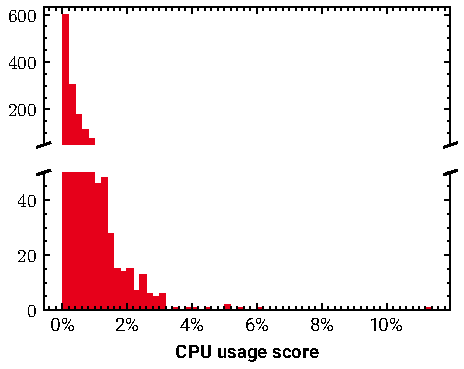
\includegraphics[width=\textwidth]{images/histogram-global.pdf}
      \caption{All web sites}
    \end{subfigure}
    \hfill
    \begin{subfigure}[t]{0.5\textwidth}
      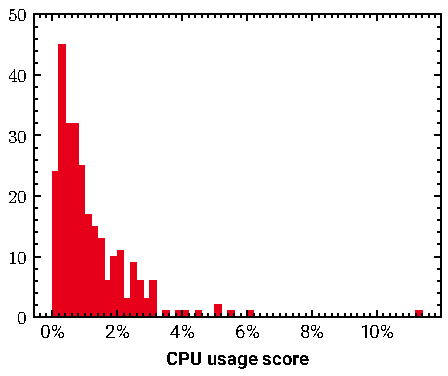
\includegraphics[width=\textwidth]{images/histogram-method.pdf}
      \caption{Only web sites using a circumvention method}
    \end{subfigure}

    \caption{Distribution of average CPU usage}
    \label{fig:distribution-cpu-usage}
  \end{figure}
  
  We manually analysed a random sample set of web sites with background execution higher than 2~\% by dissecting the corresponding trace file in the Chrome profiler. We discovered that the vast majority of background execution is attributable to advertisement and tracker scripts. We observed two main activities which are done in the background by these scripts. First, they report the user activity to their tracking server. Second, they rotate the ads displayed in the web site to record multiple ad views during one page view. Both of these activites cause several network requests which further impact the energy usage of the web site. Additionally, the tracker scripts communicate in regular intervals with the iframes in which the ads are displayed. This communication happens via \texttt{postMessage()} calls which, as we now know, is not throttled by browsers.
  
  Some news related web sites reload the complete window after a certain amount of time to show the latest content of the home page when a user leaves the tab open for a long time. This is a low effort solution to always show the current content without the need for dynamic content replacement scripts and can be easily integrated into existing content management systems. A side effect of reloading the page is that the background timer throttling is reset and the first ten seconds after the page reload are not subject to budget limits again. As these news related web site often also include third party ad network scripts, these scripts also have to be executed again. The first seconds after the page was loaded often is the most CPU intensive period during the whole runtime of the web site. During our analysis we observed that web sites reloading themselves after a certain amount of time often exceed the timer budget limits.
  
  To summarize, we did not find web sites in our sample that actively do abuse the limit circumventing methods to gain background execution. However, even though these web sites were not visible to the user, they did consume non trivial amounts of CPU time. We claim, that most of the background execution performed from these web sites were not necessary to function correctly. Web site creators should constrain the background execution of their web site to only providing functionallity expected and wanted by users.

  
  \newpage
  \chapter{Discussion and conclusion}

  As we have concluded in chapter \ref{chap:analysis}, the browser throttling mechanisms do not protect users from malicous web sites, which actively try to utilize background execution. They can only be regarded as energy conserving measures for well-behaving web sites. We also showed in chapter \ref{chap:tracing} that the circumvention methods are used by popular web sites.

  To protect users from unwanted CPU usage of background tabs, browsers should suspend tabs completely when they are not visible to the user. This goal is already acknowledged from Chrome developers as stated in \cite{chrome-background-tabs-roadmap}. The reason why this change is not yet implemented can be attributed to the missing alternative APIs for legitimate use of background timers. Suspending all background tabs would break these use cases, in which users expect the page to update in the background. Safari implemented a good interim solution by detecting high energy consumption of background tabs and terminating them when they reach a certain threshold. This solution allows web site to utilize background execution but only if it does not impact battery life too much and it protects users from continuous CPU usage and battery drain from web miners or other CPU expensive workloads.

  We propose two possible solutions to browser vendors for letting users give web sites permission to utilize continuous background exection while still suspending all other web sites:

  \begin{figure}
    \centering
    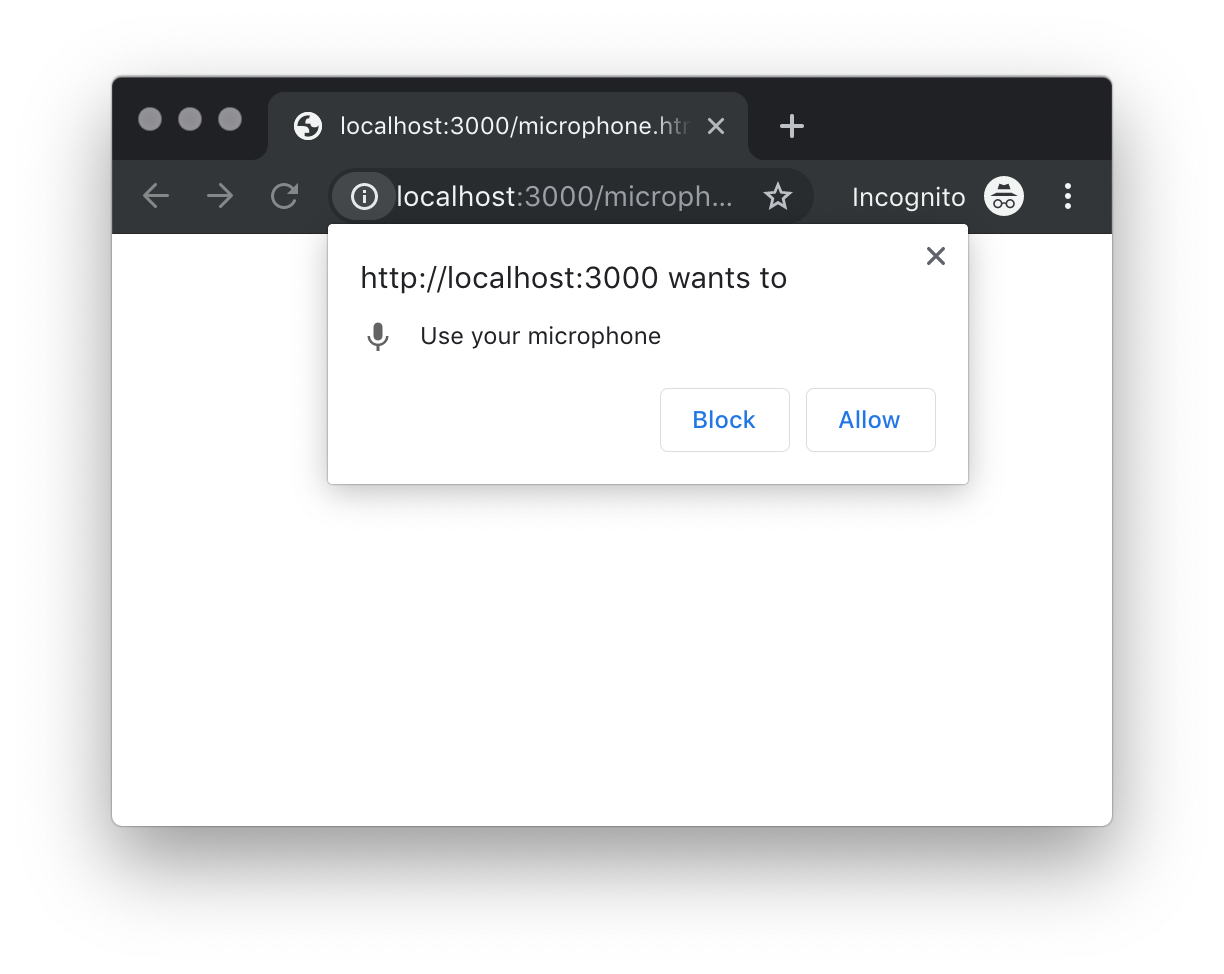
\includegraphics[width=0.5\textwidth]{images/microphone-permission.png}
    \caption{Chrome permission dialog}
    \label{fig:chrome-permission-dialog}
  \end{figure}

  The first proposed solution is to ask the user for explicit permission before the utilization of background execution is allowed for a web site requesting it. Browser could display a popup where users can allow or deny the use of background execution. This popup based permission system is already implemented for privacy concerning activities for example when a web site ask for the users location or access to camera and microphone. Figure \ref{fig:chrome-permission-dialog} shows how this popup looks like in Chrome. One could argue that even more permission popups could train users to blindly accept whatever is shown to them. This behaviour is also reinforced by numerous cookie and privacy policy dialogs as implemented to conform to the recently introduced GDPR. On the other hand, cookie and privacy policy are shown inside the web site frame, whereas the proposed background execution permission dialog should be shown from the browser UI and can therefore be recognized as a more important dialog. Web sites would then have to opt in to not to be suspended when in the background. And there is still the question of the right time for the permission popup to be shown to the user. User experience research shows, that users are more likely to deny permission for elevated access, when it is not clear to them, why these permissions are needed \cite{bonne2017exploring}. Therefore, it is considered best practice to not show the permission dialog until the permission is first needed. A good example is the microphone or camera permission dialog. Consider a video conferencing web sites where the permission dialog could be shown, when the users tries to join a call. The natural time for web sites to ask for background exection permission is when the user switches to another tab. But then, indeed, the context of the web site may already be lost and the authorization request at this time could be confusing to the user. Another obvious time would be, when the user first visits the web site. However, this behaviour contradicts the experience, that users are less likely to give permissions as soon as the web site is loaded. It may not be clear to the user at this time, why the web site needs background execution to function properly. Another approach would be to show the dialog as soon as the user refocuses the tab a couple of times after it was in the background. At that time it is confirmed that the user frequently checks the content of the web site. The permission dialog could as well explain to the user, that the content of this page does not refresh in the background without the explicit permission for background execution.

  \begin{figure}
    \centering
    
\includegraphics[width=0.5\textwidth]{images/pinned-tab.png}
    \caption{Pinned tab feature in Safari. In contrast to regular tabs, the pinned tab only shows the web sites favicon and has no close button.}
    \label{fig:pinned-tab}
  \end{figure}
  
  The second proposed solution is to disable suspension of tabs, when they are pinned. Pinned tabs is a feature implemented by most desktop browsers, which allows easy access to frequently used web sites. Figure \ref{fig:pinned-tab} shows how a pinned tab looks like in Safari. \cite{firefox-pinned-tabs} explains how pinned tabs work in Firefox. It also describes, why users should use pinned tabs: ``The internet is now full of websites that we use more like programs than just static pages. Popular sites like Facebook and Gmail are like this – they're used to accomplish tasks (or to avoid accomplishing tasks), they update themselves and notify you when they've changed.'' Web sites, which users are likely to pin, are oftentimes the same pages benefiting from background execution. It therefore makes sense to combine the permission for background execution to pinned tabs. We claim that the coupling of the background execution permission and pinned tabs is exactly what users expect for pinned tabs. With this solution, users do not have to be asked for another permission and it allows legitimate web sites to perform background tasks while still letting the user be in control of background execution. Additionally, it would not require a new API for requesting the background execution permission and is therefore backwards compatible with existing web sites. Pinning a web site tab thereby converts the browser behaviour from a normal web site to a web application.

  Mobile browsers do not have a concept of pinned tabs, but Android and iOS support adding web sites to the home screen. When added to the home screen, a web site can hide the browser UI for navigation and the address bar to behave more like a fully native application. We propose to give background execution permission to these web sites which were added to the home screen by the user. This would be the equivalent of a pinned tab on desktop browsers for background execution behaviour.
  
  
  \newpage
  \printbibliography[heading=bibnumbered]


  \affidavit


\end{document}
%%% Local Variables: 
%%% mode: latex 
%%% TeX-engine: luatex
%%% TeX-master: t 
%%% End: